\documentclass[10pt,a4paper]{book}
\usepackage{amsmath, graphicx, hyperref}
\graphicspath{{figures/}}

\title{A Laboratory Course on Single Molecule Localization Microscopy}

\author{Kyle M. Douglass}

\date{\today}

\begin{document}

\maketitle

\chapter{Introduction}

\section{Super-Resolution Fluorescence Microscopy}

Fluorescence microscopy is a set of techniques that allows scientists to study the structure and behavior of microscopic systems. Cell biologists in particular use fluorescence microscopes to visualize biological systems across many different spatial scales, from macromolecular complexes, organelles, and cells to tissues and even whole organisms. The power of fluorescence microscopy comes from the ability to label specific molecules with fluorescent markers such that the presence of light coincides with the presence of the target molecules. This molecular specificity, when combined with a light microscope's ability to magnify specimens that are normally too small to see with the unaided eye, provides a powerful tool to better understand the microscopic world.

All light microscopes, however, are bound by the laws of diffraction which state that the smallest features that can be observed by the instrument are approximately the size of the wavelength of light. Anything smaller than this so-called diffraction limit appears blurred, often to the point where an observer is completely unable to infer its structure from an image. For biologists this is particularly problematic because many important cellular structures have sizes that are smaller than this limit.

Starting in the 1900s researchers began to discover ways to circumvent the diffraction limit of light microscopy and image structures that were smaller than a wavelength with good fidelity. Among the first such techniques that was proposed and realized was the near-field optical microscope, whereby a sample is scanned by an illuminated aperture that is smaller than the wavelength of light. Unfortunately, this technique is somewhat cumbersome to use for cell biology studies because of the constraints that the instrument places on the sample. In the early 1990s it was discovered that the resolution of confocal fluorescence microscopes, a standard instrument in cell biology, could be improved beyond the diffraction limit by up to a factor of two and still remain compatible with biological samples.\footnote{Resolution, as we shall see, is often defined as the smallest distance at which two very small light emitters may be located with respect to one another and still be determined to be separate objects.} Several new techniques quickly followed, such as stimulated emission depletion (STED) microscopy, structured illumination (SIM) microscopy, and photoactivated localization microscopy (PALM). All of these techniques, which collectively would come to be called super-resolution microscopy, were compatible with the requirements of biologists. Additonally, the plethora of techniques present different tradeoffs in terms of spatiotemporal resolutions, signal-to-noise ratios, and live-cell compatibilities so that today's cell biologist can choose the instrument that best suits their needs.

In this course you will learn about a super-resolution fluorescence microscopy technique called \textbf{single molecule localization microscopy}, or SMLM. SMLM uses light to stochasticly manipulate photophysical states of fluorescent molecules such that the images of individual molecules can be located with high precision, often on the order of tens of nanometers. A set of location estimates recorded across time (called localizations), are combined to form an image with a resolution that surpasses the diffraction limit of light. SMLM has been used to study a number of celluar structures and processes, such as the diffusion of membrane proteins, axonal actin rings, the nuclear pore complex, and centrioles.

\section{Learning Outcomes}

\begin{enumerate}
    \item Explain how a modern epifluorescence microscope works, including a list of its main components and their relationships to one another.
    \item Identify the main components of an epifluorescence microscope on the real microscope in the lab.
    \item Explain the principle behind single molecule localization microscopy and how it overcomes the diffraction limit of light.
    \item Model fluorescence phenomena such as photoswitching and photoactivation as continuous-time Markov chains.
    \item Analyze data from the microscope to produce super-resolved images of cellular structures.
\end{enumerate}

\chapter{The Modern Fluorescence Microscope}

\section{Epifluorescence Microscopes}

The design of a modern fluorescence microscope is illustrated in \autoref{fig:epifluorescence-microscope}. In this design, light from a source such as a laser or a high intensity LED enters the microscope and is reflected into the objective lens by a dichroic mirror.\footnote{A dichroic mirror is a mirror with an engineered surface that reflects some wavelengths of light and transmits others.} The exictation light is focused by the objective lens onto the sample where it excites fluorescent molecules within the sample. The fluorescence light is collected by the same objective and passes subsequently through the dichroic mirror. A second lens, known as the tube lens, collects the fluorescence light and forms an image of the sample on the camera.

\begin{figure}[ht]
    \centering
    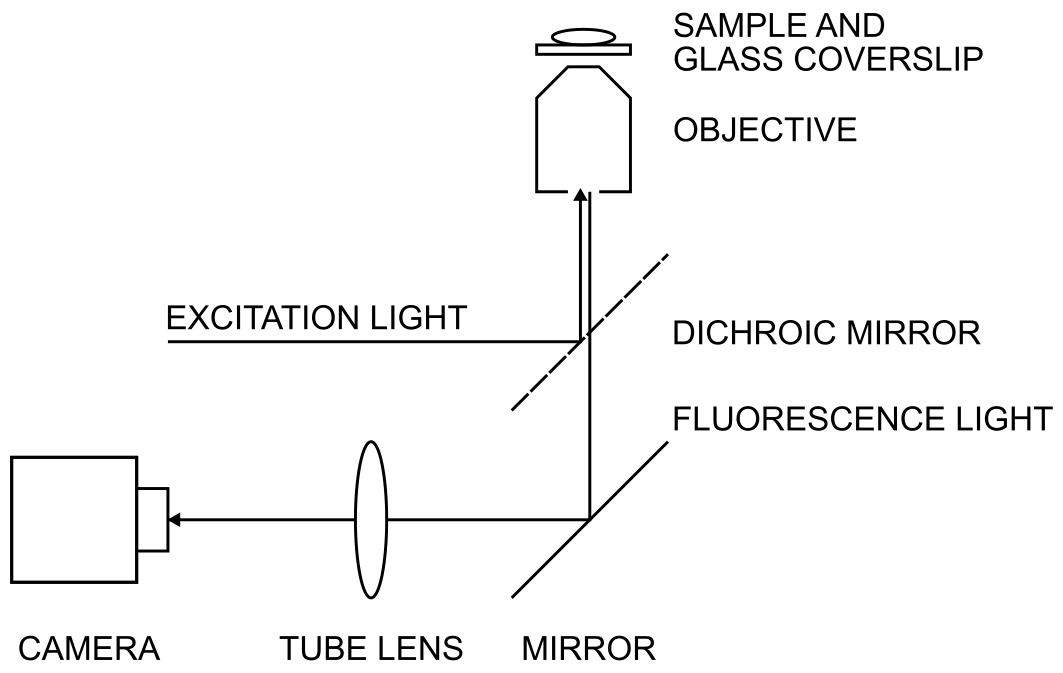
\includegraphics{epifluorescence-microscope.png}
    \caption{Principle components of an infinity corrected epifluorescence microscope.}
    \label{fig:epifluorescence-microscope}
\end{figure}

There are a few important things to understand about this microscope. The first is that the choices for light source, dichroic mirror, and fluorophore are not completely independent.\footnote{This is true for all fluorescence microscopes, not just for the design being discussed here.} The reason for this is largely due to a fluorophore's Stokes shift, or the difference between the excitation light wavelength and the fluorescence wavelength. As a result of this difference, the choice of fluorophore will determine the wavelength of the light source that is necessary. It will also determine the so-called passband of the dichroic mirror; it must be selected so that sufficient amounts of excitation light is reflected and fluorescence light is transmitted. If the dichroic mirror is poorly chosen, either not enough light will illuminate the sample or not enough fluorescence photons will be detected (or both). In practice, the passbands of dichroic mirrors are standardized around a few popular fluorphores, such as green fluorescent protein (GFP).

Another important characteristic of the design illustrated in \autoref{fig:epifluorescence-microscope} is that the sample is excited by the same lens that collects the fluorescence signal. This geometry is known as \textbf{epi-illumination}, as opposed to \textbf{transillumination} whereby the sample is illuminated by light that is focused onto the sample by a separate condenser lens. When imaging fluorescence from a sample and simply reflected light, it is known more specifically as \textbf{epifluorescence}. Epifluorescence microscopes solve the problem of the excitation light dominating the weaker fluorescence signal because most of the excitation light propagates away from the objective after it leaves the sample.

\section{Infinity Corrected Systems}

A final thing to note about the design in \autoref{fig:epifluorescence-microscope} is that the final image of the sample is formed on the camera by a second lens called the tube lens. Modern microscope objectives are infinity corrected. As illustrated in \autoref{fig:infinity-space}, an infinity corrected system places the sample in the front focal plane of the objective lens. The result is that the image of the sample is formed at infinity after the objective and requires the tube lens to form a real image at the camera's sensor plane.

\begin{figure}[ht]
    \centering
    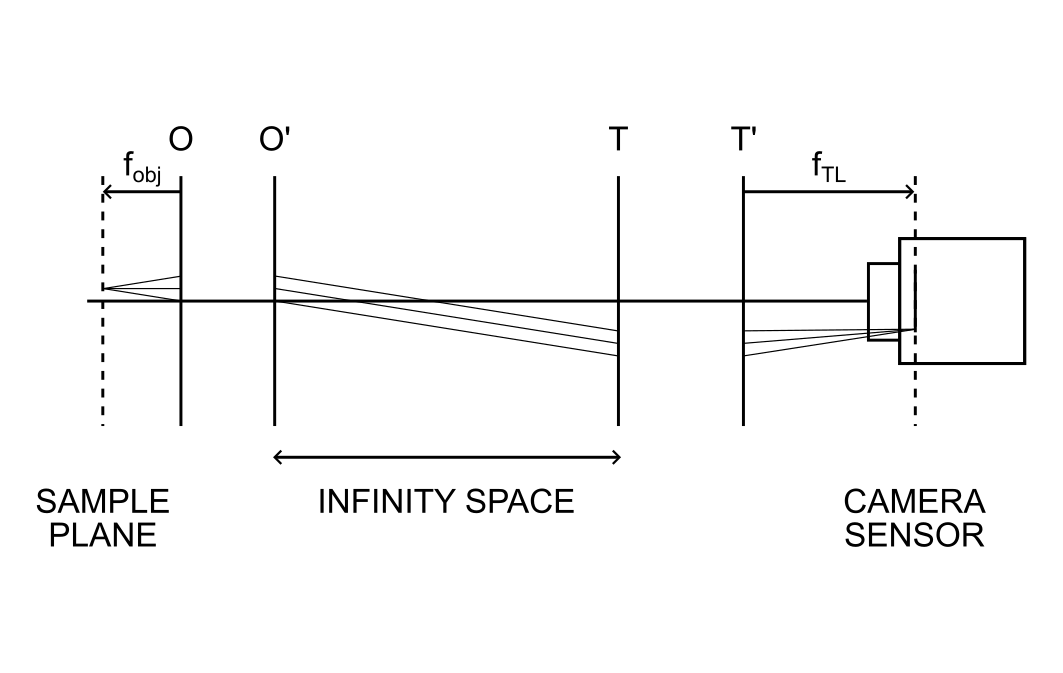
\includegraphics{infinity-space.png}
    \caption{Optical path of an infinity corrected microscope. Rays emitted from a point in the sample plane are parallel in the infinity space. $O/O'$ and $T/T'$ denote the principle planes of the objective and tube lens, respectively. $f_{obj}$ and $f_{TL}$ denote their focal lengths.}
    \label{fig:infinity-space}
\end{figure}

Prior to the development of infinity corrected systems, microscope objectives formed their images at a fixed distance from the objective, called the tube length. By convention, this distance was usually around 160 mm. A second lens, the eye piece, would reform the image for viewing by an observer. Modern microscopy often requires that additonal optical elements be placed after the objective during measurements, such as dichroic mirrors and filters. Upon insertion into the optical path, one of these additonal elements would displace the location of the image formed by a traditional objective due the refractive index difference between the element's material and air. This in turn would force the microscopist to refocus the image and result in a slightly different magnification of the final image. Infinity corrected systems do not suffer from these problems because the intermediate image is located at infinity. As a result, the final image will not change the position when additonal elements are inserted into the so-called infinity space between the objective and tube lens.

\section{Imaging Properties of Microscopes}

\subsection{The Point Spread Function}

One of the most useful tools to characterize the performance of a microscope is the \textbf{point spread function}, or PSF. Qualitatively, the PSF is the image formed by the microscope of an infinitesimally small object emitting light uniformly in all directions. A microscope without aberrations\footnote{An aberration is any deformation of the PSF other than that caused by diffraction.} will have a PSF that is well-modeled by the Airy disk, which is the pattern seen in \autoref{fig:airy-pattern}.

\begin{figure}[ht]
    \centering
    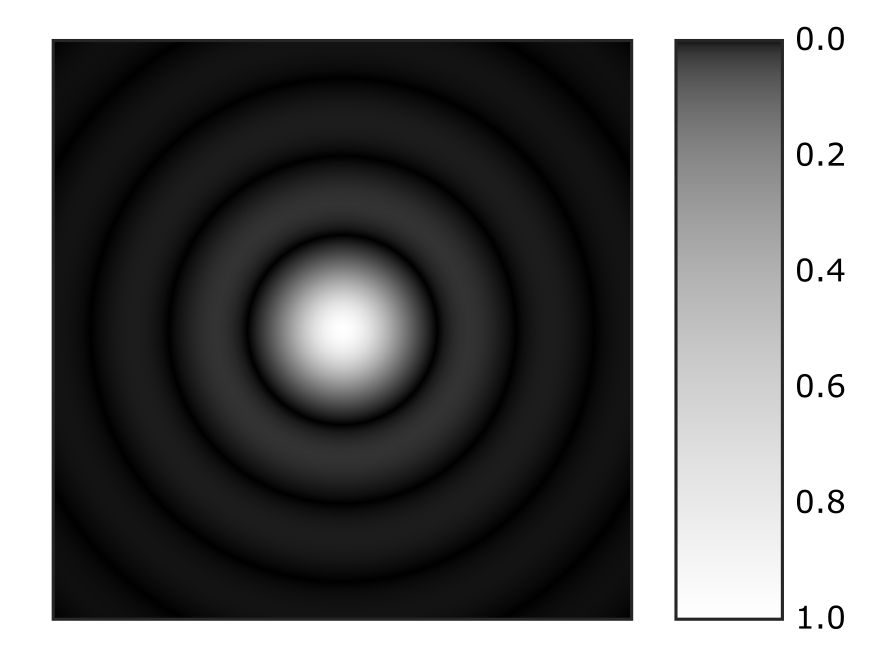
\includegraphics{Airy-pattern.png}
    \caption{The Airy disk pattern. Lighter colors denote regions of higher light intensity. By Sakurambo at English Wikipedia - Public Domain, \url{https://commons.wikimedia.org/w/index.php?curid=18640280}.}
    \label{fig:airy-pattern}
\end{figure}

The expression for the Airy disk is derived from scalar diffraction theory, i.e. the polarization of light is ignored. More precisely, it is the Fraunhofer diffraction pattern of a uniformly-illuminated circular aperture.\footnote{This is identical to solving for the image of an isotropically-emitting, incoherent point source because such a source uniformly fills the system's pupil.} Mathematically, the expression is

\begin{equation}
    I \left(X\right) = I_{0} \left[ \frac{2 J_{1}\left(X\right)}{X} \right]^2
\end{equation}

\noindent where $ X = 2 \pi r \text{NA} / \lambda $, $r$ is the radial coordinate in the image plane, $\text{NA}$ is the numerical aperture of the microscope, and $\lambda$ is the wavelength of light. $J_{1}\left(X\right)$ is called the first-order Bessel function of the first kind. Its first zero, which is important for defining resolution as we shall see later, is at $\Delta X = 3.8317$. In terms of the radial coordinate, it lies at $\Delta r \approx 0.61 \text{NA} / \lambda$.

\subsection{Image Formation in Linear Shift Invariant Systems}

Since the PSF is by definition the image of an infinitesimally small emitter and because it has a finite spatial extent, it follows that the PSF is a measure of the blurring of the image of an object seen through a microscope due to diffraction. But what about samples containing many fluorophores? How does the point spread function affect its image?

We can answer this question if we first assume a few properties about the microscope. The first is linearity, i.e. the image of two fluorophores is just the sum of the image of each fluorophore individually. The second assumption is that the microscope is shift invariant. This means that the PSF does not depend on the location of an emitter. 

Let the density of fluorescence emitters in a plane be represented by $O \left(x, y\right)$. Under the two assumptions above\footnote{These assumptions are equivalent to those used to model linear time invariant systems, which are characterized by an impulse response. The PSF is analogous to the impulse response.}, the resulting image $I \left(x, y\right)$ is the convolution of this density with the PSF $h \left(x, y\right)$, or

\begin{equation}
    I \left(x, y\right) = h \left(x, y\right) \ast O \left(x, y\right)
\end{equation}

We can reduce the degree of blurring by increasing the numerical aperture of the objective, which has the effect of reducing the size of the PSF. Ultimately, however, diffraction prevents us from shrinking the PSF down to a point. As a result, a microscope image will never exactly reproduce an image of the object.

\chapter{Single Molecule Localization Microscopy}

\section{Determination of a Single Molecule's Position}

We saw in the previous chapter that diffraction determines the size of the smallest object that can be seen through a microscope. This size is approximately equal to half of the wavelength of light, which for visible wavelengths is approximately 250 nm.

Under some conditions, however, we can actually determine the location of single fluorescent molecules to a precision that is roughly 10 times better than the diffraction limit, or on the order of 10 nm. This process is called localizing a molecule, and the resulting estimate of its position is called a localization. The technique to do this is called single molecule localization microscopy, or SMLM.

To understand how SMLM works, let's first consider a sample that consists of a single fluorescent molecule. When excited with light, the molecule emits fluorescence and the microscope will record a blurred image of the molecule. Such an image is shown in figure XXX.

The key insight of SMLM is that the position of the molecule is located at the center of its image, and we can find the center to high precision. To do this, we fit a model of the image of a single molecule to the image recorded by the microscope. Two of the model parameters will be the $x$ and $y$ positions of the molecule's center. Thus the result of the fit is an estimate of the molecule's position. 


\chapter{Fluorescence Photophysics}

\chapter{Localization Microscopy in Practice}

\begin{figure}[ht]
    \centering
    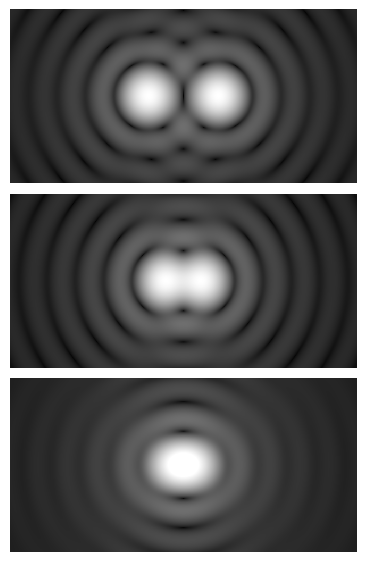
\includegraphics[width=0.75\textwidth]{Airy_disk_spacing_near_Rayleigh_criterion.png}
    \caption{Rayleigh criterion}
    \label{fig:rayleigh}
\end{figure}

\end{document}
